\section{Results}
The complete results are published on \href{https://github.com/diogorrio/discovering_fm_for_treewidth}{this} GitHub repository, under the package 'docs/results'. Ideally, as the algorithm is run, the said package is updated accordingly. The graphs are available through their database file, if the user chooses to see the edge lists that define the minimal forbidden minors themselves. In addition, image representations are provided.

\subsection{Some Found Minimal Forbidden Minors}
In this section, some of the found minimal forbidden minors are displayed. It should be noted that some graphs are more symmetrically drawn than others. Several design layouts were tested, and the subjectively clearest out of each of them was chosen.

\subsubsection{The Known: Small Treewidth}
The algorithm managed to \textit{exclusively} find all the minimal forbidden minors for treewidth 1, 2, and 3. That means the program did not identify any incorrect minors and instead found all the already known ones, for small treewidths.
\vspace{0.5cm}

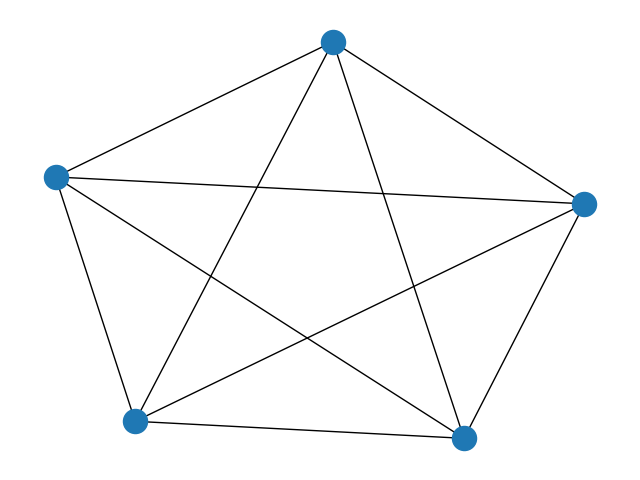
\includegraphics[width=3.2cm]{images/mfms/k5.png}
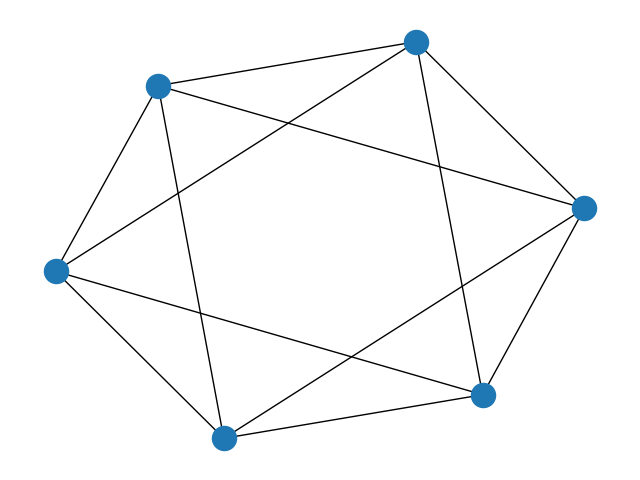
\includegraphics[width=3.2cm]{images/mfms/octahedron.png}
\vskip\baselineskip
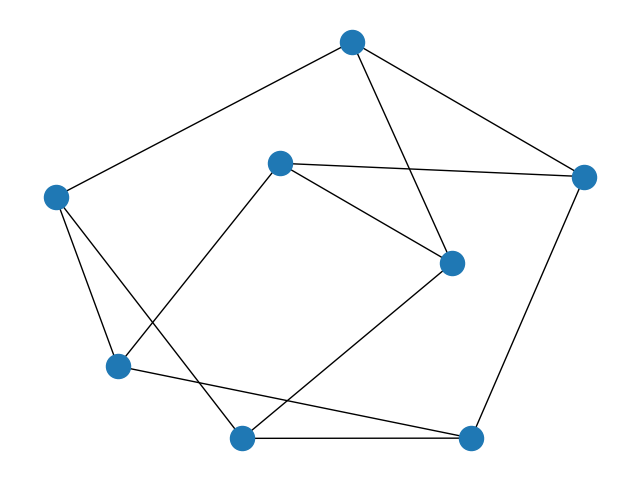
\includegraphics[width=3.2cm]{images/mfms/wagner.png}
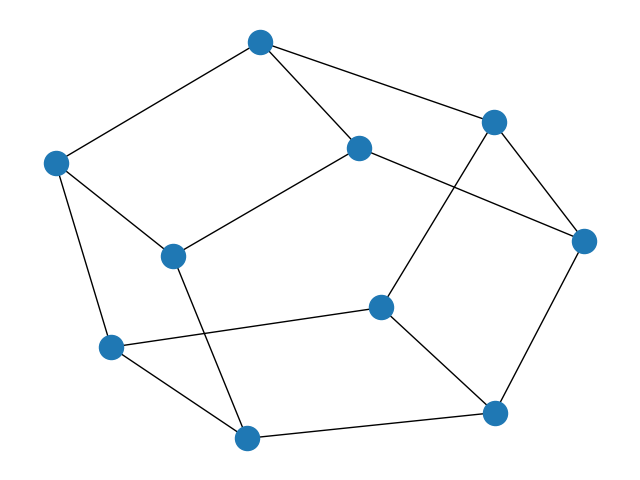
\includegraphics[width=3.2cm]{images/mfms/pentagonal_prism.png}  
\begin{center}
  \captionof{figure}{The 4 MFMs of $F(3)$: $K_5$, the octahedron, Wagner's graph, and the pentagonal prism (top left to bottom right).}
\end{center}

\subsubsection{The Unknown: \textit{F(4)}}
Here are some of the 41 found minimal forbidden minors for $k=4$.
\vspace{0.5cm}

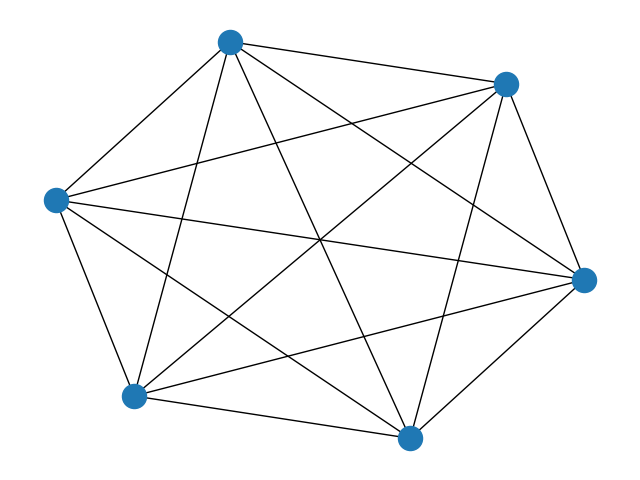
\includegraphics[width=3.2cm]{images/mfms/f4_1.png}
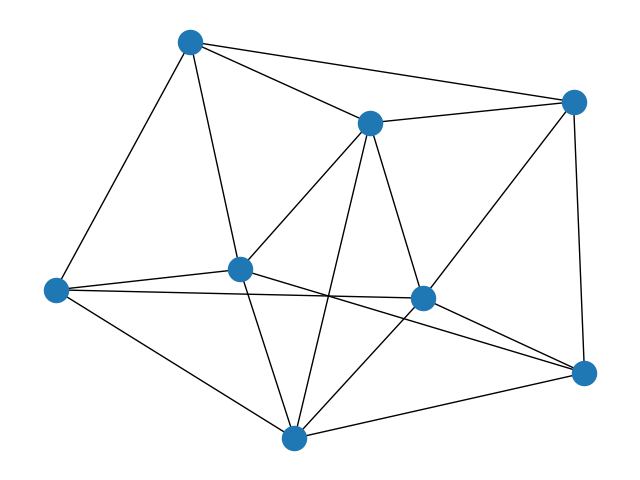
\includegraphics[width=3.2cm]{images/mfms/f4_3.png}
\vskip\baselineskip
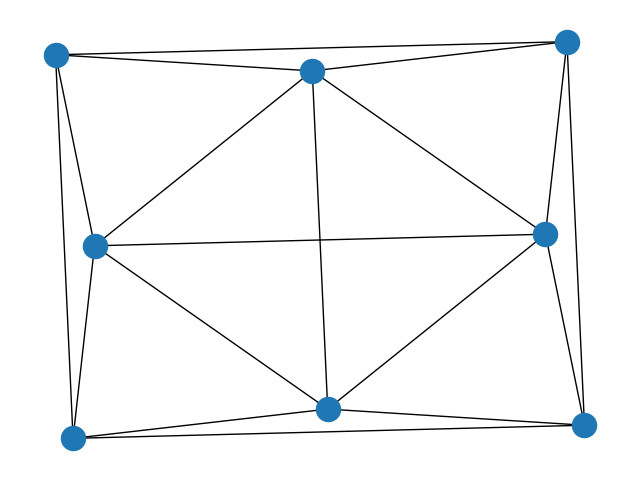
\includegraphics[width=3.2cm]{images/mfms/f4_5.png}
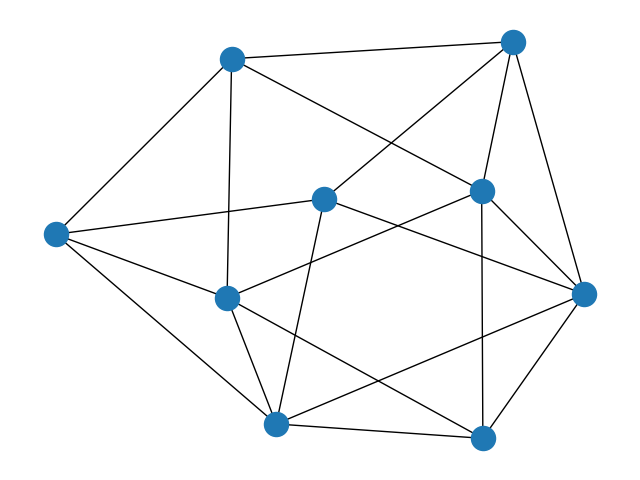
\includegraphics[width=3.2cm]{images/mfms/f4_9.png}

\subsubsection{The Unknown: \textit{F(5)}}
The number of minimal forbidden minors found for $F(5)$ is significantly smaller than that of what was the main focus of this thesis, $F(4)$. The time spent on this set was therefore limited,  contrary to $k=4$, which was the primary goal. Nonetheless, some of the 4 found minimal forbidden minors for $k=5$ are here presented as well. Displaying the graphs with a circular layout helps understand the differences between minors as they grow more complex.
\vspace{0.5cm}

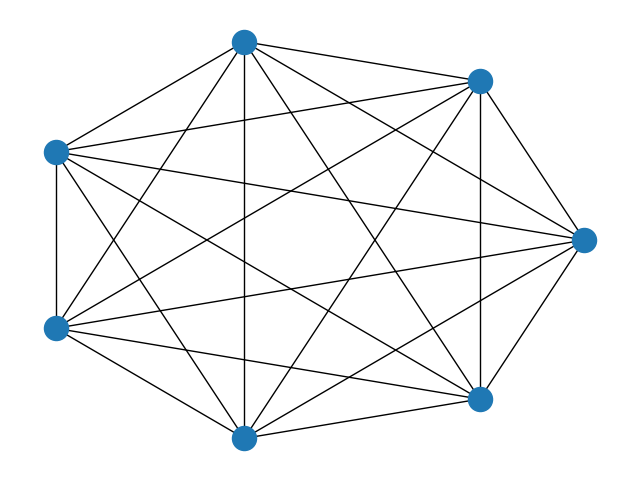
\includegraphics[width=3.2cm]{images/mfms/f5_1.png}
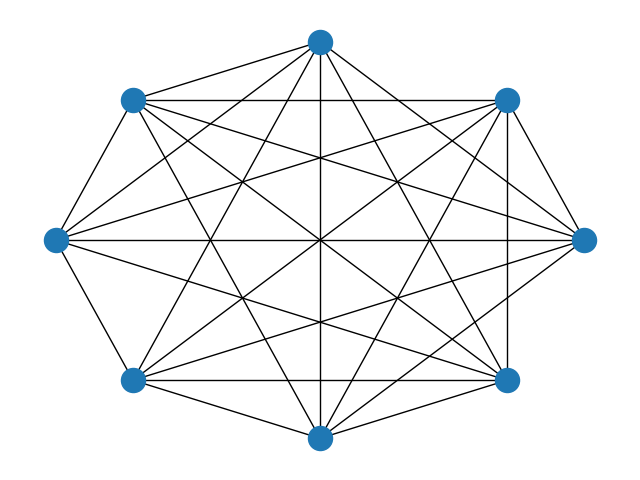
\includegraphics[width=3.2cm]{images/mfms/f5_2.png}
